\documentclass[xcolor=dvipsnames,14pt,professionalfonts]{beamer}
\usepackage{minted}
\usepackage{etoolbox}
\usepackage[T1]{fontenc}
\usepackage{lmodern}
\usepackage[no-math]{fontspec} 
\usetheme{rsmarttraining}
\usefonttheme{professionalfonts}
\usecolortheme{dolphin}

%\definecolor{foreground}{gray}{0}
%\definecolor{background}{gray}{1}
%\definecolor{keyword}{rgb}{0.2,0.2,0.8}
%\definecolor{warning}{rgb}{0.8,0.2,0.2}
%\definecolor{shadow}{gray}{0.35}
%\definecolor{hide}{gray}{0.9}
%\definecolor{figure}{rgb}{1,0.7,0}
%\definecolor{title}{rgb}{25,240,250}
\definecolor{title}{rgb}{0.09,0.30,0.38}
\definecolor{frametitle}{rgb}{1,1,1}
\definecolor{normal}{rgb}{0,0,0}

%\usecolortheme[named=keyword]{structure}

\setbeamercolor{title}{fg=title}
\setbeamercolor{frametitle}{fg=frametitle}
\setbeamercolor{section in toc}{fg=foreground}
\setbeamercolor{normal text}{bg=brown!46,fg=normal}

\setbeamerfont{structure}{family=\fontspec{Georgia},series=\bfseries} 
\setbeamerfont{subtitle}{family=\fontspec{Helvetica},series=\bfseries} 
\begin{document}

\title{KRAD Training}
\subtitle{Exercise: Maintenance Documents Part 3}
\author[Leo]{Leo Przybylski}

\usebackgroundtemplate%
{%
    
\includegraphics[width=\paperwidth,height=\paperheight]{../img/header.png}%
}

{
\usebackgroundtemplate{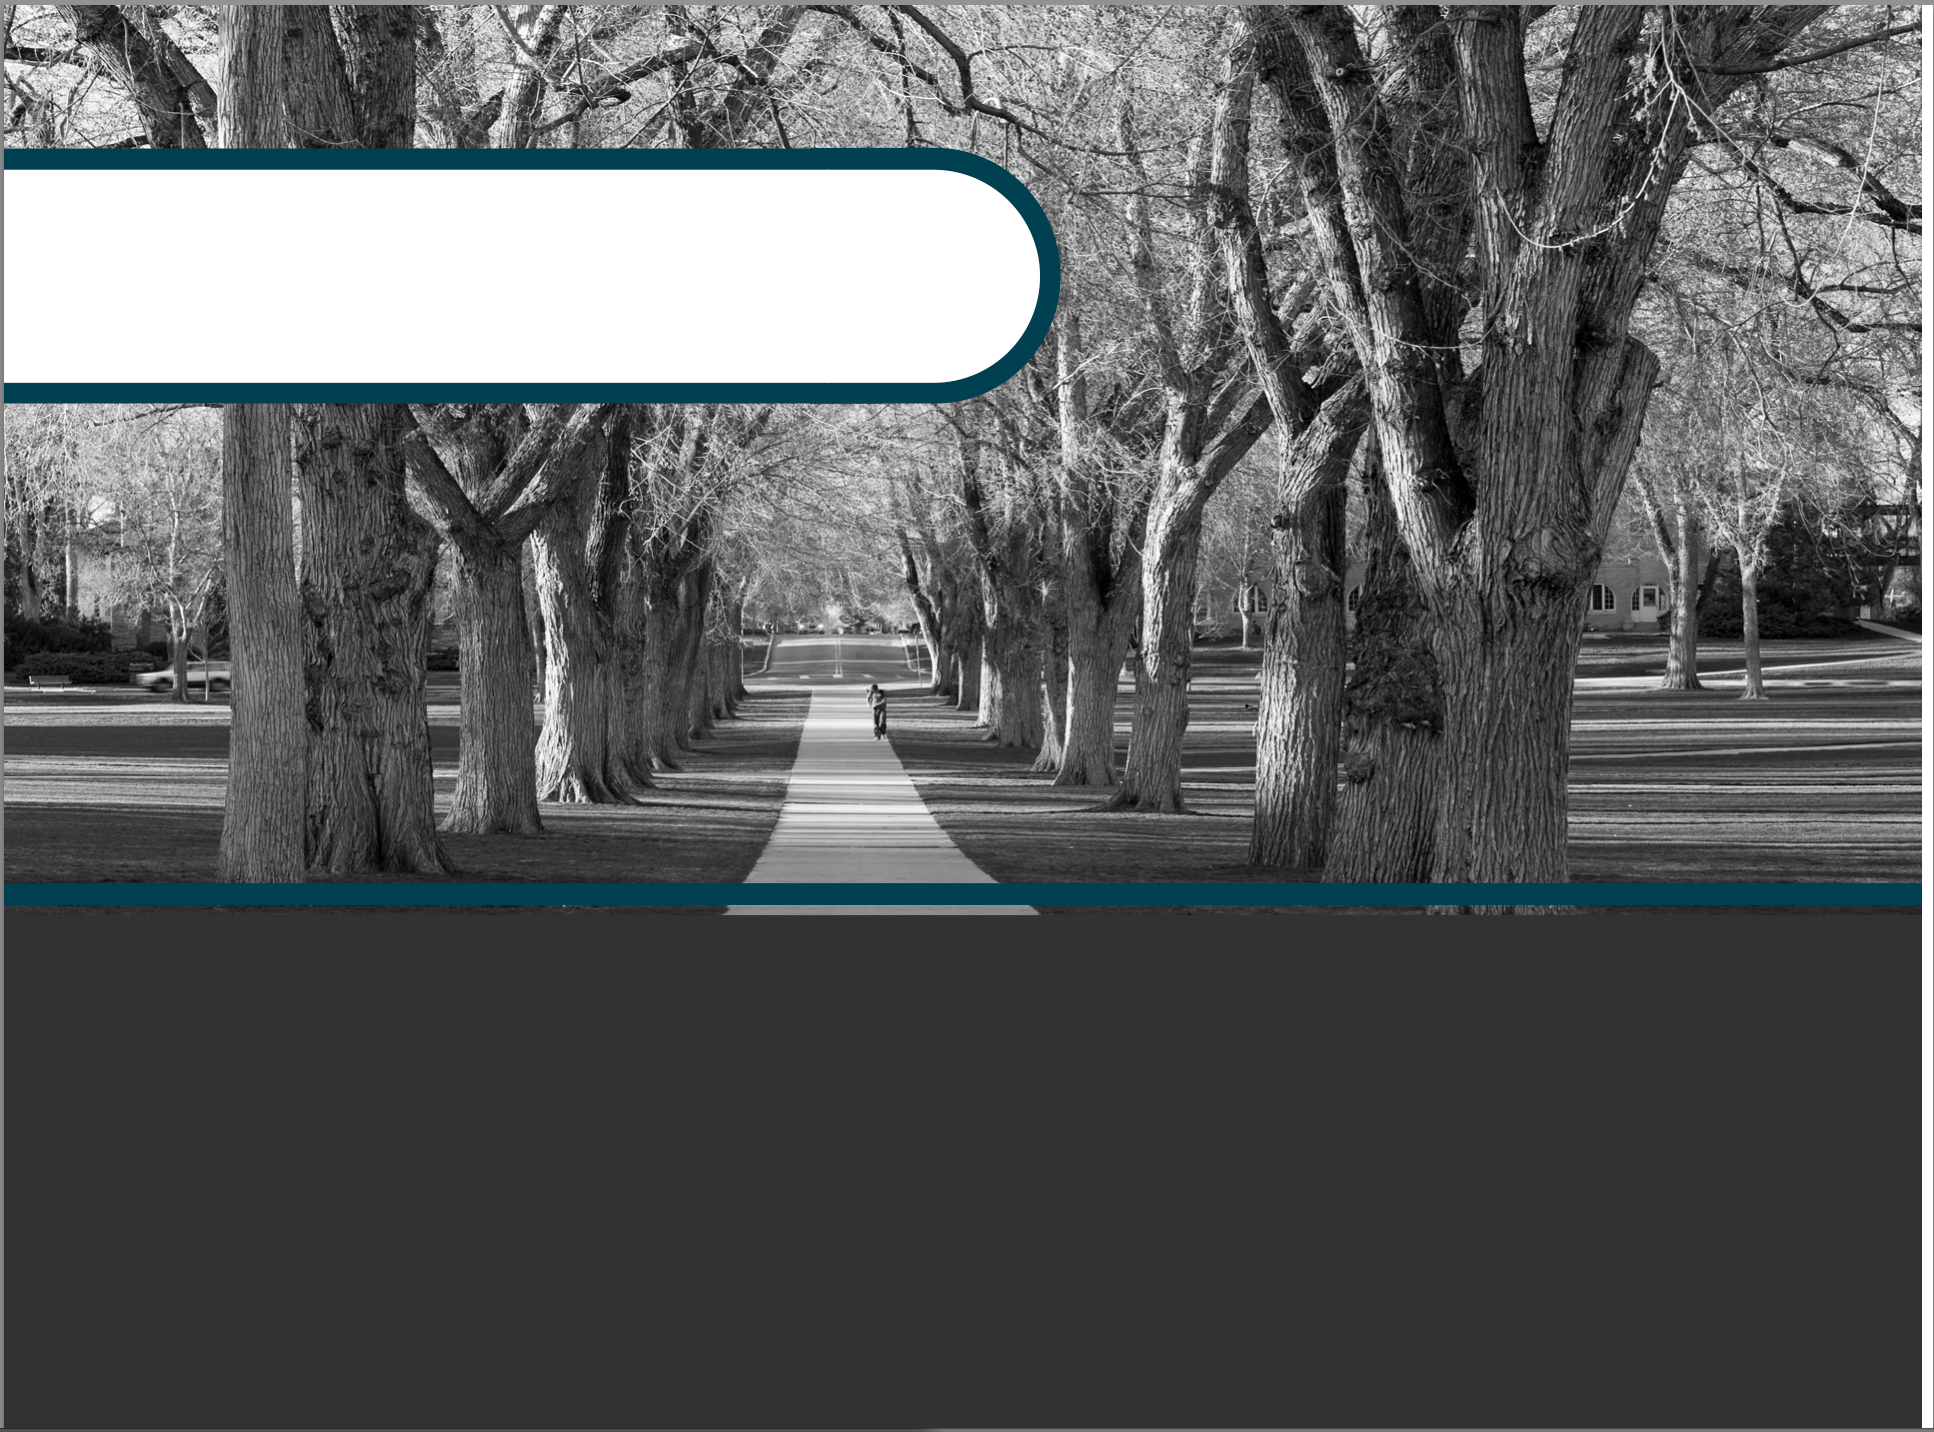
\includegraphics[width=\paperwidth]{../img/title.png}}%
\begin{frame}[plain]
  \titlepage
\end{frame}
}

\begin{frame}{Goals}
  \begin{itemize}
 \item Learn how defining a Maintenance Document Collections and how
   to work with business objects have have one to many relationships.
 \item Implement a Collection for the Book maintenance document.
\end{itemize}
\end{frame}

\begin{frame}{Checkout “exercise-krad-maint-collection” project}
  \begin{itemize}
    \item To ensure a clean and consistent environment for everyone, we will check out a project from Subversion as a starting point.  This will essentially be a completed copy of the previous exercises.
    \item In order to get the copy of the project that you will need,
      please check out the \textbf{exercise-krad-maint-collection} project from
      the training Subversion repository.
      \end{itemize}
    \end{frame}
    
    \begin{frame}{Create Chapter DataObject}
      \begin{itemize}
      \item We are going to create a one-to-many relationship within
        the Book. The Book will have Chapters. To do this we need to
        create a Chapter DataObject.
      \item We need 4 things for this:
        \begin{enumerate}
          \item Database table
          \item Java class
          \item O/R mapping
          \item DataDictionary entry
          \end{enumerate}
      \end{itemize}     
    \end{frame}

    \begin{frame}{Create chapter_t table}
 To do this, follow these steps:
      \begin{itemize}
      \item The source code has been included for this. Just as in
        other exercises, execute the \texttt{chapter.sql} file within
        the included \texttt{workflow} folder.
      \end{itemize}     
    \end{frame}
 
 \begin{frame}{Create Chapter Java Class}
   Just as with other DataObjects, we will need a \texttt{Chapter}
   java class. Create one in \textbf{trnapp.bookstore}. Add the
   following properties to it.
   \begin{itemize}
     \item id
     \item title
     \item number
     \item bookId
   \end{itemize}
 \end{frame}

 \begin{frame}[fragile]{Add Reference to Chapter}
   Next we need to reference the \texttt{Chapter} from the
   \texttt{Book}. It's a one-to-many relationship, so there needs to
   be a Collection of chapters in \texttt{Book}
 \begin{minted}[fontsize=\scriptsize]{java}
    final List<Chapter> chapters;
    
    public Book() {
        chapters = new ArrayList<Chapter>();
    }
    \end{minted}
\end{frame}
   

 \begin{frame}{Create a DataDictionary Entry}
   Likewise, we also need a DataDicationary Entry. Make sure you have
   attributes for the following:
   \begin{itemize}
     \item id
     \item title
     \item number
     \item bookId
   \end{itemize}
 \end{frame}

 \begin{frame}{Create O/R Mapping}
   We need to create our mapping between the Chapter class and the
   chapter_t table. The sample is in the next slide.
 \end{frame}

 \begin{frame}[fragile]{Create O/R Mapping}
 \begin{minted}[fontsize=\scriptsize]{xml}
<class-descriptor class="trnapp.bookstore.Chapter" table="chapter_t">
    <field-descriptor name="id" column="chapter_id" jdbc-type="BIGINT" 
        primarykey="true" autoincrement="true" sequence-name="chapter_s" />
    <field-descriptor name="title" column="title" jdbc-type="VARCHAR" />
    <field-descriptor name="number" column="number" jdbc-type="INTEGER" />
    <field-descriptor name="bookId" column="book_id" jdbc-type="BIGINT" />
    <field-descriptor name="objectId" column="obj_id" jdbc-type="VARCHAR" />
    <field-descriptor name="versionNumber" column="ver_nbr" 
    jdbc-type="BIGINT" locking="true" />
</class-descriptor>
    \end{minted}
\end{frame}

 \begin{frame}[fragile]{Create O/R Mapping}
Now there needs to be a one-to-many reference in the mapping. To do
this, we add the following collection-descriptor to the Book mapping.
 \begin{minted}[fontsize=\scriptsize]{xml}
<collection-descriptor name="chapters" 
    collection-class="org.apache.ojb.broker.util.collections.ManageableArrayList"
    element-class-ref="trnapp.bookstore.Chapter"
    proxy="true'' auto-retrieve="false" auto-update="true" auto-delete="true">
    <inverse-foreignkey field-ref="bookId" />
</collection-descriptor>
    \end{minted}
\end{frame}

    \begin{frame}{Add Maintenance Collection}
     \begin{itemize}
       \item We can't forget the whole purpose which is to add a
         collection to a maintenance document. 
       \item We now need to update the BookMaintenanceDocument.xml to
         add chapters to it.
       \item The example is on the next slide.
      \end{itemize}     
    \end{frame}

 \begin{frame}[fragile]{Add Maintenance Collection}
 \begin{minted}[fontsize=\scriptsize]{xml}
<bean parent="Uif-MaintenanceTableCollectionSection">
    <property name="headerText" value="Chapters" />
    <property name="collectionObjectClass" value="trnapp.bookstore.Chapter" />
    <property name="propertyName" value="chapters" />           
    <property name="items">
      <list>
         <bean parent="Uif-InputField" p:label="Number" p:propertyName="number"/>
         <bean parent="Uif-InputField" p:label=''Title" p:propertyName="title"/>
      </list>
    </propery>
</bean>      
    \end{minted}
\end{frame}
           
\end{document}
